
\documentclass[12pt]{article}
\usepackage[margin = 1in]{geometry}
\usepackage[dvipsnames]{xcolor}
\usepackage{tabularx}
\usepackage{graphicx}
\usepackage{enumitem}
\usepackage{hyperref}
% \usepackage{fancyhdr}
\usepackage[margin = 0cm]{caption}
\usepackage{wrapfig}
\usepackage{amsmath}
\usepackage{amssymb}
\usepackage{natbib}
\setlength{\bibsep}{0pt}
\hypersetup{ % all blue links
	colorlinks		= true,
	urlcolor 		= blue,
	linkcolor 		= blue,
	citecolor 		= blue
}
\setcitestyle{aysep={}, yysep={,}}
\newcommand{\aj}{AJ}
\newcommand{\aap}{A\&A}
\newcommand{\aapr}{A\&ARv}
\newcommand{\apj}{ApJ}
\newcommand{\apjl}{ApJL}
\newcommand{\apjs}{ApJS}
\newcommand{\apss}{Ap\&SS}
\newcommand{\araa}{ARA\&A}
\newcommand{\baas}{BAAS}
\newcommand{\fcp}{Fundamentals Cosmic Phys.}
\newcommand{\mnras}{MNRAS}
\newcommand{\nat}{Nature}
\newcommand{\pasa}{PASA}
\newcommand{\pasp}{PASP}
\newcommand{\ddfrac}[2]{\frac{\displaystyle{#1}}{\displaystyle{#2}}}
\newcommand{\msun}{\ensuremath{\text{M}_\odot}}
\newcommand{\scinote}[2]{\ensuremath{#1\times10^{#2}}}
\providecommand{\noopsort}[1]{}

\newcommand{\ah}{\ensuremath{\text{[$\alpha$/H]}}}
\newcommand{\mh}{\ensuremath{\text{[M/H]}}}
\newcommand{\timescale}[1]{\ensuremath{\tau_\text{#1}}}
\newcommand{\harmonic}[2]{\ensuremath{\bar{\tau}_\text{[#1,#2]}}}
\newcommand{\hharmonic}[3]{\ensuremath{\bar{\tau}_\text{[#1,#2,#3]}}}
\renewcommand{\tilde}[1]{\ensuremath{\widetilde{#1}}}

\begin{document}

\begin{center}
\textbf{The Shape and Centroid of Abundance Distributions for Inside-Out Star
Formation Histories in One-Zone Models}
\par\null\par
James W. Johnson
\par\null\par
\rule[0.7\baselineskip]{0.5\textwidth}{0.4pt}
\end{center}

\par\noindent
The motivating question is the origin of the Galactic abundance gradient in the
context of Galactic winds.
Galactic chemical evolution (GCE) models like that of~\citet{Johnson2021}
invoke strong mass loading to explain the observed abundances with yields
predicted by stellar evolution models.
Consequently, each Galactic region quickly reaches some equilibrium abundance
where metal production by young stars is balanced by losses to outflows, and
the gradient arises out of a decrease in the equilibrium abundance with
increasing radius.
However, in models like that of~\citet*{Minchev2013, Minchev2014} and
\citet{Spitoni2019}, the authors neglect mass loading in the outflowing
material, and therefore the equilibrium abundance does not vary with radius.
Both classes of models successfully reproduce the observed gradient, but this
is by construction in the~\citet{Johnson2021} models.
This begs the question as to which parameter choices must be made in order to
successfully reproduce this empirical result in the latter class of models.
\par
To this end, here I derive analytic and parametric expressions for the
metallicity distribution function (MDF) given a set of choices of GCE model
parameters.
The MDF in the metal mass fraction~$Z$ can be expressed as:
\begin{equation}
\frac{dN}{dZ} = \frac{dN}{dt} \bigg/ \frac{dZ}{dt}
\propto \frac{\dot{M}_\star}{\dot{Z}},
\label{eq:dndz}
\end{equation}
where~$\dot{M}_\star$ is the star formation rate (SFR).
In general,~$\dot{M}_\star$ and~$\dot{Z}$ will be parametric functions of time.
As a consequence of the abundance gradient, the mode of the MDF shifts from
metal-rich to metal-poor with increasing radius
\citep[see, e.g.,][]{Hayden2015}.
Therefore, it is also interesting to estimate the position of the maximum in
the MDF by taking its derivative and setting it equal to zero:
\begin{subequations}\begin{align}
\frac{d^2N}{dZ^2} &= \frac{d}{dZ} \left(\frac{dN}{dZ}\right)
\\
&= \frac{1}{\dot{Z}} \frac{d}{dt} \left(\frac{dN}{dZ}\right)
\\
&\propto \frac{1}{\dot{Z}} \frac{d}{dt}
\left(\frac{\dot{M}_\star}{\dot{Z}}\right)
\\
&= \frac{1}{\dot{Z}} \left(\frac{
	\dot{Z}\ddot{M}_\star - \ddot{Z}\dot{M}_\star
}{
	\dot{Z}^2
}\right)
\\
&= \frac{\dot{M}_\star}{\dot{Z}^2}
\left(\frac{\ddot{M}_\star}{\dot{M}_\star} - \frac{\ddot{Z}}{\dot{Z}}\right).
\label{eq:d2ndz2}
\end{align}\end{subequations}
By setting the above expression equal to zero, it is apparent that maxima in the
MDF in~$Z$ occurs when
\begin{equation}
\frac{\ddot{M}_\star}{\dot{M}_\star} = \frac{\ddot{Z}}{\dot{Z}}.
\label{eq:zmdf_maxima_criterion}
\end{equation}
\par
In practice, however, abundances are quantified logarithmically.
It is therefore also interesting to compute the MDF in~\mh,\footnote{
	I adopt standard notation where~$\mh \equiv \log_{10}(Z / Z_/\odot) -
	\log_{10}(X / X_\odot)$ where~$Z_\odot$ is the metal mass fraction of the
	sun and~$X$ and~$X_\odot$ are the corresponding hydrogen mass fractions.
	However, since hydrogen mass fractions do not vary much (especially when
	scalled logarithmically), here I assume that~$\log_{10}(X / X_\odot)
	\approx 0$ and therefore~$\mh \approx \log_{10}(Z / Z_\odot)$.
} which is straight-forward given the derivations already written out above.
The MDF in~\mh~itself:
\begin{equation}
\frac{dN}{d\mh} = \ln 10 \left(\frac{Z}{Z_\odot}\right) \frac{dN}{dZ}
\propto \frac{\dot{M}_\star}{\dot{Z} / Z},
\label{eq:dndmh}
\end{equation}
and its derivative:
\begin{subequations}\begin{align}
\frac{d^2N}{d\mh^2} &= \frac{d}{d\mh} \left(\frac{dN}{d\mh}\right)
\\
&= \ln 10 \left(\frac{Z}{Z_\odot}\right) \frac{d}{dZ}
\left(\ln 10 \frac{Z}{Z_\odot} \frac{dN}{dZ}\right)
\\
&= \left(\frac{\ln 10}{Z_\odot}\right)^2 Z\frac{d}{dZ}
\left(Z\frac{dN}{dZ}\right)
\\
&= \left(\frac{\ln 10}{Z_\odot}\right)^2
Z\left(\frac{dN}{dZ} + Z\frac{d^2N}{dZ^2}\right)
\\
&= \left(\frac{\ln 10}{Z_\odot}\right)^2 \left(Z\frac{dN}{dZ} +
Z^2 \frac{d^2N}{dZ^2}\right)
\\
&\propto \frac{\dot{M}_\star}{\dot{Z} / Z} +
\frac{\dot{M}_\star}{(\dot{Z} / Z)^2}
\left(\frac{\ddot{M}_\star}{\dot{M}_\star} - \frac{\ddot{Z}}{\dot{Z}}\right).
\label{eq:d2ndmh2}
\end{align}\end{subequations}
By setting equation~\ref{eq:d2ndmh2} equal to zero, it then follows that maxima
in the MDF in~\mh~occur when
\begin{equation}
\frac{\ddot{M}_\star}{\dot{M}_\star} = \frac{\ddot{Z}}{\dot{Z}} -
\frac{\dot{Z}}{Z}.
\label{eq:mhmdf_maxima_criterion}
\end{equation}
\par
For the remainder of this document, I derive solutions to the above expressions
for the ``inside-out'' star formation history (SFH) from~\citet{Johnson2021}:
\begin{equation}
\dot{M}_\star(t) \propto \left(1 - e^{-t / \timescale{rise}}\right)
e^{-t / \timescale{sfh}}.
\label{eq:insideout_sfh}
\end{equation}
The physically interesting advantage of this parameterization over the classic
``linear-times-exponential''~$t e^{-t / \timescale{sfh}}$ form is that the
rise timescale~\timescale{rise}~gives one some control over how long the SFH is
increasing independent of~\timescale{sfh}.
In the interest of analytic/parametric solutions, I assume that the star
formation efficiency (SFE) timescale~$\tau_\star \equiv M_\text{g} /
\dot{M}_\star$ and the outflow mass loading factor~$\eta \equiv
\dot{M}_\text{out} / \dot{M}_\star$ are both constant in time.
In the interest of simplicity, I also focus on alpha elements with negligible
yields from Type Ia supernovae (e.g., O and Mg), and I adjust my notation
accordingly from~$Z$ to~$Z_\alpha$ and~\mh~to~\ah~hereafter.

\par\null\par\noindent
\textbf{Analytic solution to~$Z_\alpha(t)$}
\par\noindent
The expression for~$\dot{M}_\star$ is given by the assumption of equation
\ref{eq:insideout_sfh}, so now I must solve for~$Z_\alpha(t)$ using arguments
similar to those of~\citet*{Weinberg2017}.
For alpha elements,~\citet*{Weinberg2017} express the rate of change of the
mass present in the ISM as
\begin{equation}
\dot{M}_\alpha = y_\alpha \dot{M}_\star - Z_\alpha \dot{M}_\star (1 + \eta - r),
\label{eq:mdot_alpha}
\end{equation}
where~$y_\alpha$ is a population-averaged alpha element yield from massive
stars, assumed to be ejected immediately after a stellar population forms.
This assumption is valid due to the short lifetimes of massive stars compared
to the relevant evolutionary timescales of the Milky Way.
$r$ is a term which accounts for the return of stellar envelopes back to
the ISM ($r \approx 0.4$ for a~\citealt{Kroupa2001} IMF;
\citealp*{Weinberg2017}).
\par
Based on the definition of~$Z_\alpha$, the quotient rule implies that its
time-derivative can be expressed as
\begin{subequations}\begin{align}
\dot{Z}_\alpha &= \frac{
	M_\text{g} \dot{M}_\alpha - M_\alpha \dot{M}_\text{g}
}{
	M_\text{g}^2
}
\\
&= \frac{
	M_\text{g} (y_\alpha \dot{M}_\star - Z_\alpha \dot{M}_\star (1 + \eta - r))
	- M_\alpha \ddot{M}_\star \tau_\star
}{
	M_\text{g}^2
}
\\
&= y_\alpha \frac{\dot{M}_\star}{M_\text{g}} -
Z_\alpha \frac{\dot{M}_\star}{M_\text{g}}(1 + \eta - r) -
Z_\alpha \frac{\ddot{M}_\star}{M_\text{g}} \tau_\star
\\
&= \frac{y_\alpha}{\tau_\star} -
Z_\alpha \left(\frac{1 + \eta - r}{\tau_\star} +
\frac{\ddot{M}_\star}{\dot{M}_\star}\right).
\label{eq:dzdt}
\end{align}\end{subequations}
The next step is to differentiate the SFH with time to compute
$\ddot{M}_\star / \dot{M}_\star$. Taking~$A$ to denote the overall normalizing
factor:
\begin{subequations}\begin{align}
\ddot{M}_\star &= \frac{d}{dt}
A(1 - e^{-t / \timescale{rise}}) e^{-t / \timescale{sfh}}
\\
&= A \frac{1}{\timescale{rise}}e^{-t / \timescale{rise}}
e^{-t / \timescale{sfh}} +
A(1 - e^{-t / \timescale{rise}}) \frac{-1}{\timescale{sfh}}
e^{-t / \timescale{sfh}}
\\
&= A(1 - e^{-t / \timescale{rise}})e^{-t / \timescale{sfh}}
\left(\frac{
	e^{-t / \timescale{rise}}
}{
	\timescale{rise}(1 - e^{-t / \timescale{rise}})
} - \frac{1}{\timescale{sfh}}
\right)
\\
\implies \frac{\ddot{M}_\star}{\dot{M}_\star} &= \frac{
	e^{-t / \timescale{rise}}
}{
	\timescale{rise}(1 - e^{-t / \timescale{rise}})
} - \frac{1}{\timescale{sfh}}.
\label{eq:mddotstar-over-mdotstar}
\end{align}\end{subequations}
At this point, it is straightforward to compute the equilibrium alpha element
abundance for this SFH by plugging equation~\ref{eq:mddotstar-over-mdotstar}
into equation~\ref{eq:dzdt} and setting~$\dot{Z}_\alpha = 0$.
This procedure results in the following expression:
\begin{equation}
Z_{\alpha,\text{eq}} = \ddfrac{
	y_\alpha
}{
	1 + \eta - r + \frac{
		\tau_\star e^{-t / \timescale{rise}}
	}{
		\timescale{rise}(1 - e^{-t / \timescale{rise}})
	} - \frac{\tau_\star}{\timescale{sfh}}
}.
\label{eq:zalpha-eq}
\end{equation}
Equation~\ref{eq:zalpha-eq} indicates that unlike the simpler SFHs like a
constant or single exponential, the equilibrium abundance is not uniform in
time.
Instead, the term in the denominator depending on~\timescale{rise} is infinite
at~$t = 0$.
Therefore, the equilibrium abundance is zero at~$t = 0$, increases at early
times, and then approaches the solution for a single exponential
once~$t \gg \timescale{rise}$.
As a sanity check, equation~\ref{eq:zalpha-eq} indeed reduces to the
equilibrium abundance for a single exponential SFH found
by~\citet*{Weinberg2017} if I let~$\timescale{rise} \rightarrow 0$.
\par
Plugging this into equation~\ref{eq:dzdt} above yields the following linear
ODE for~$Z_\alpha$:
\begin{equation}
\dot{Z}_\alpha + Z_\alpha \left(\frac{1}{\timescale{dep}} +
\frac{
	e^{-t / \timescale{rise}}
}{
	\timescale{rise}(1 - e^{-t / \timescale{rise}})
} - \frac{1}{\timescale{sfh}}\right) = \frac{y_\alpha}{\tau_\star},
\end{equation}
where I have substituted for the depletion time, defined as
$\timescale{dep} \equiv \tau_\star / (1 + \eta - r)$.
$\timescale{dep}$ quantifies the e-folding timescale on which the ISM would
decline due to both star formation and mass loading, if present.
For notational convenience, I define the function~$f(t)$ to denote the
multiplicative factor on~$Z_\alpha$:
\begin{equation}
f(t) \equiv \frac{1}{\timescale{dep}} + \frac{
	e^{-t / \timescale{rise}}
}{
	\timescale{rise}(1 - e^{-t / \timescale{rise}})
} - \frac{1}{\timescale{sfh}},
\end{equation}
such that the general solution for~$Z_\alpha$ can be expressed as
\begin{equation}
Z_\alpha(t) = \exp\left(-\int f(t') dt'\right)\left(
\int_0^t \exp\left(\int f(t') dt'\right) \frac{y_\alpha}{\tau_\star} dt' + C
\right),
\label{eq:za-linear-ode}
\end{equation}
where the constant~$C$ will later be assigned such that the initial
condition~$Z_\alpha(t = 0) = 0$ is satisfied.
At this point, it is helpful to zoom in on the integral of~$f(t)$.
Its term depending on~$\timescale{rise}$ can be integrated with a series of
variable substitutions:
\begin{subequations}\begin{align}
\int \frac{
	e^{-t / \timescale{rise}}
}{
	\timescale{rise}(1 - e^{-t / \timescale{rise}})
} dt
&= \int \frac{e^{-u}}{1 - e^{-u}} du
\qquad \left(u = \frac{t}{\timescale{rise}};~~du = \frac{1}{\timescale{rise}}
dt\right)
\\
&= \int \frac{dv}{v} \qquad \left(v = 1 - e^{-u};~~dv = e^{-u} du\right)
\\
&= \ln v
\\
&= \ln (1 - e^{-u})
\\
&= \ln (1 - e^{-t / \timescale{rise}})
\\
\implies \int f(t) dt
&= \frac{t}{\timescale{dep}} + \ln (1 - e^{-t / \timescale{rise}}) -
\frac{t}{\timescale{sfh}}.
\end{align}\end{subequations}
Solving equation~\ref{eq:za-linear-ode} amounts to integrating the sum of a
handful of exponentials with prefactors that depend on~\timescale{rise},
\timescale{dep}, and~\timescale{sfh} in a non-trivial way.
The full derivation is attached, and the final solution is given by
\begin{equation}
\begin{split}
Z_\alpha(t) &= \frac{1}{1 - e^{-t / \timescale{rise}}}
\left(\frac{y_\alpha}{1 + \eta - r}\right)
\bigg[\frac{
	\timescale{sfh}
}{
	\timescale{sfh} - \timescale{dep}
} \left(
1 - \exp\left(-t\frac{
	\timescale{sfh} - \timescale{dep}
}{
	\timescale{sfh}\timescale{dep}
}\right)
\right) -
\\
&\qquad \frac{
	\timescale{sfh}\timescale{rise}
}{
	\timescale{sfh}\timescale{rise} - \timescale{dep}\timescale{rise} -
	\timescale{sfh}\timescale{dep}
} \left(e^{-t / \timescale{rise}} -
\exp\left(-t
\frac{
	\timescale{sfh} - \timescale{dep}
}{
	\timescale{sfh}\timescale{dep}
}
\right)
\right)\bigg].
\end{split}
\end{equation}
Adopting the harmonic timescale notation~$\harmonic{X}{Y} = \timescale{Y}
\timescale{X} / (\timescale{Y} - \timescale{X})$ of~\citet*{Weinberg2017}
simplifies the expression:
\begin{equation}
\begin{split}
Z_\alpha(t) &= \frac{1}{1 - e^{-t / \timescale{rise}}} \left( \frac{
	y_\alpha
}{
	1 + \eta - r
}\right) \bigg[
\frac{\harmonic{dep}{sfh}}{\timescale{dep}}
\left(1 - e^{-t / \harmonic{dep}{sfh}}\right) -
\\
&\qquad \frac{\hharmonic{dep}{rise}{sfh}}{\timescale{dep}}
\left(e^{-t / \timescale{rise}} - e^{-t / \harmonic{dep}{sfh}}\right)
\bigg]
\end{split}
\label{eq:zalpha}
\end{equation}
\par
At~$t = 0$, the factor~$1 / (1 - e^{-t / \timescale{rise}})$ is infinite,
but the factor enclosed in square brackets is zero.
Therefore, a physical solution exists if and only if the integration
constant~$C$, included in the full derivation of this expression (see equation
\ref{eq:zalpha-full}), is equal to zero.
Because this results in the~$\infty \times 0$ indeterminate form, I can simply
define the abundance to be zero such that the boundary condition
of~$Z_\alpha(t = 0) = 0$ is satisfied.

\begin{figure*}
\centering
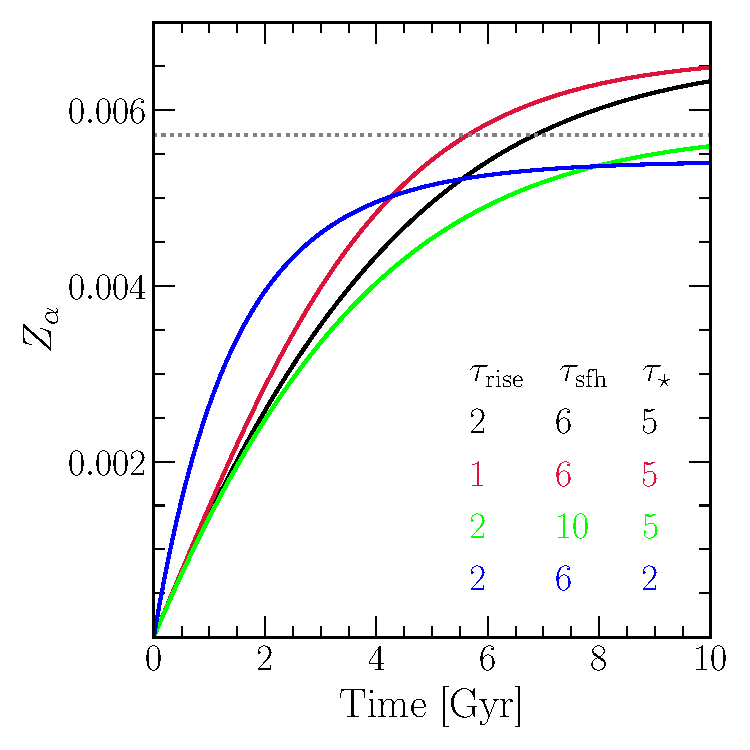
\includegraphics[scale = 0.52]{vartimescales.pdf}
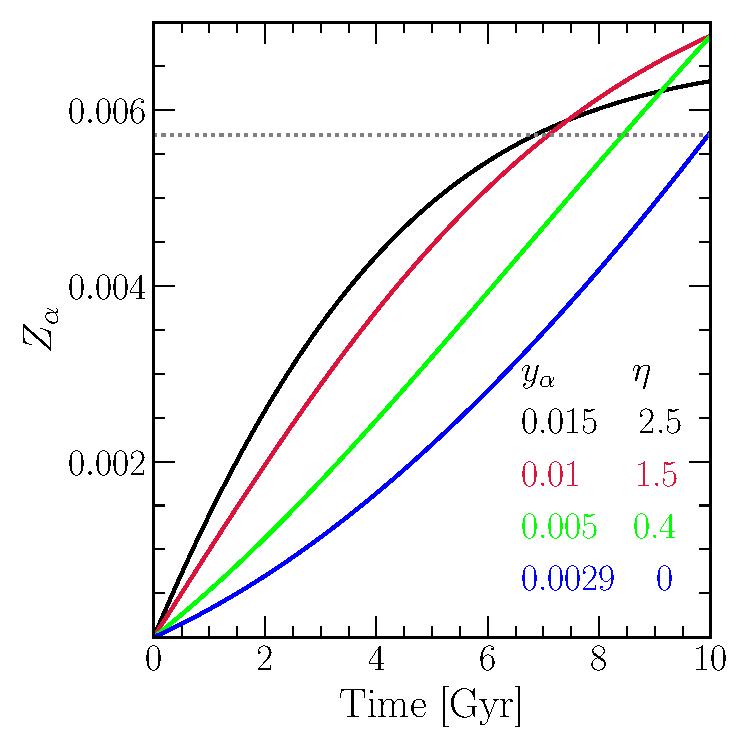
\includegraphics[scale = 0.52]{varyieldeta.pdf}
\caption{
Analytically computed evolution in the oxygen abundance according to equation
\ref{eq:zalpha}.
\textbf{Left}: For~$y_\alpha = 0.015$ and~$\eta = 2.5$, each curve denotes a
different choice of some timescale.
With black visualizing a fiducial choice of parameters of (\timescale{rise},
\timescale{sfh},~$\tau_\star$) = (2 Gyr, 6 Gyr, 5 Gyr), crimson shows a short
rise timescale (i.e.,~$\timescale{rise} = 1$ Gyr), lime green shows a more
extended SFH (i.e.,~$\timescale{sfh} = 10$ Gyr), and blue shows a higher SFE
(i.e.,~$\tau_\star = 2$ Gyr).
\textbf{Right}: For the fiducial choice of timescales in the right-hand panel,
each curve denotes a different choice of~$y_\alpha$ and~$\eta$ as denoted in
the legend.
For each choice of~$y_\alpha$, the value of~$\eta$ is chosen such that the
ratio~$y_\alpha / (1 + \eta - r)$ is approximately constant, and vice versa in
the case of the blue line where I choose~$\eta = 0$ and compute the
corresponding value of~$y_\alpha$.
}
\label{fig:analytic-evolution}
\end{figure*}

The left panel of Fig.~\ref{fig:analytic-evolution} visualizes the evolution of
the alpha element abundances according to equation~\ref{eq:zalpha} under
different choices of timescales.
% A shorter rise timescale has the effect of raising the abundances overall
\par
The right panel of Fig.~\ref{fig:analytic-evolution} visualizes the enrichment
history for the fiducial choice of timescales in the left panel, but with
different values of~$y_\alpha$ and~$\eta$, selected such that the value of
$y_\alpha / (1 + \eta - r)$ is approximately constant.
\par\null\par\noindent
\textbf{The Time-Derivative of~$Z_\alpha(t)$}
\par\noindent
The differentiate~$Z_\alpha(t)$ with time, it compactifies notation to define
some function~$g(t)$ denoting the term in square brackets in equation
\ref{eq:zalpha}:
\begin{equation}
g(t) \equiv \frac{\harmonic{dep}{sfh}}{\timescale{dep}}
\left(1 - e^{-t / \harmonic{dep}{sfh}}\right) -
\frac{\hharmonic{dep}{rise}{sfh}}{\timescale{dep}}
\left(e^{-t / \timescale{rise}} - e^{-t / \harmonic{dep}{sfh}}\right),
\label{eq:g}
\end{equation}
such that the expression for~$Z_\alpha$ reduces to
\begin{equation}
Z_\alpha(t) = \frac{1}{1 - e^{-t / \timescale{rise}}}
\left(\frac{y_\alpha}{1 + \eta - r}\right) g(t),
\end{equation}
and its time-derivative can then be obtained with product-rule:
\begin{subequations}\begin{align}
\dot{Z}_\alpha(t) &= \left(\frac{y_\alpha}{1 + \eta - r}\right)\left[
\frac{
	-e^{-t / \timescale{rise}}
}{
	\timescale{rise} \left(1 - e^{-t / \timescale{rise}}\right)^2
} g(t) + \frac{1}{1 - e^{-t / \timescale{rise}}} \dot{g}(t)
\right]
\\
&= \frac{1}{1 - e^{-t / \timescale{rise}}}
\left(\frac{y_\alpha}{1 + \eta - r}\right) g(t)
\left[
\frac{
	-e^{-t / \timescale{rise}}
}{
	\timescale{rise} \left(1 - e^{-t / \timescale{rise}}\right)
} + \frac{\dot{g}(t)}{g(t)}\right]
\label{eq:zdotalpha}
\\
\implies \frac{\dot{Z}_\alpha(t)}{Z_\alpha(t)} &=
\frac{\dot{g}(t)}{g(t)} - \frac{
	e^{-t / \timescale{rise}}
}{
	\timescale{rise} \left(1 - e^{-t / \timescale{rise}}\right)
}.
\label{eq:zdotalpha_over_zalpha}
\end{align}\end{subequations}
The time-derivative of~$g(t)$ is straight-forward:
\begin{subequations}\begin{align}
\begin{split}
\dot{g}(t) &= \frac{\harmonic{dep}{sfh}}{\timescale{dep}}
\left(0 - e^{-t / \harmonic{dep}{sfh}} \frac{-1}{\harmonic{dep}{sfh}}\right) -
\\
&\qquad \frac{\hharmonic{dep}{rise}{sfh}}{\timescale{dep}}
\left(e^{-t / \timescale{rise}}\frac{-1}{\timescale{rise}} -
e^{-t / \harmonic{dep}{sfh}} \frac{-1}{\harmonic{dep}{sfh}}\right)
\end{split}
\\
&= \frac{e^{-t / \harmonic{dep}{sfh}}}{\timescale{dep}} +
\frac{\hharmonic{dep}{rise}{sfh}}{\timescale{dep}}
\left(\frac{e^{-t / \timescale{rise}}}{\timescale{rise}} -
\frac{e^{-t / \harmonic{dep}{sfh}}}{\harmonic{dep}{sfh}}\right)
\label{eq:gdot}
\\
\implies \frac{\dot{g}(t)}{g(t)} &= \ddfrac{
	e^{-t / \harmonic{dep}{sfh}} + \hharmonic{dep}{rise}{sfh}
	\left(\frac{e^{-t / \timescale{rise}}}{\timescale{rise}} -
	\frac{e^{-t / \harmonic{dep}{sfh}}}{\harmonic{dep}{sfh}}\right)
}{
	\harmonic{dep}{sfh}\left(1 - e^{-t / \harmonic{dep}{sfh}}\right) -
	\hharmonic{dep}{rise}{sfh}\left(e^{-t / \timescale{rise}} -
	e^{-t / \harmonic{dep}{sfh}}\right)
}.
\label{eq:gdot_over_g}
\end{align}\end{subequations}
Between equations~\ref{eq:zdotalpha},~\ref{eq:zdotalpha_over_zalpha},
\ref{eq:gdot}, and~\ref{eq:gdot_over_g}, the full solution
to~$\dot{Z}_\alpha(t)$ and~$\dot{Z}_\alpha(t) / Z_\alpha(t)$ is specified.

\par\null\par\noindent
\textbf{The Second Time-Derivative of~$Z_\alpha(t)$}
\par\noindent
Differentating~$\dot{Z}_\alpha(t)$ with time follows from
equation~\ref{eq:zdotalpha}, though it simlifies things somewhat to instead
start from equation~\ref{eq:zdotalpha_over_zalpha}:
\begin{subequations}\begin{align}
\ddot{Z}_\alpha(t) &= \frac{d}{dt} \left[Z_\alpha(t) \left(
\frac{\dot{g}(t)}{g(t)} - \frac{
	e^{-t / \timescale{rise}}
}{
	\timescale{rise} \left(1 - e^{-t / \timescale{rise}}\right)
}\right)\right]
\\
&= \dot{Z}_\alpha(t) \left(\frac{\dot{g}(t)}{g(t)} - \frac{
	e^{-t / \timescale{rise}}
}{
	\timescale{rise} \left(1 - e^{-t / \timescale{rise}}\right)
}\right) + Z_\alpha(t) \frac{d}{dt} \left(\frac{\dot{g}(t)}{g(t)} - \frac{
	e^{-t / \timescale{rise}}
}{
	\timescale{rise} \left(1 - e^{-t / \timescale{rise}}\right)
}\right)
\\
\begin{split}
&= Z_\alpha(t) \Bigg[
\left(\frac{\dot{g}(t)}{g(t)} - \frac{
	e^{-t / \timescale{rise}}
}{
	\timescale{rise} \left(1 - e^{-t / \timescale{rise}}\right)
}\right)^2 + \frac{
	g(t) \ddot{g}(t) - \dot{g}(t)^2
}{
	g(t)^2
} -
\\
&\qquad \frac{
	e^{-t / \timescale{rise}}
}{
	\timescale{rise}^2 \left(1 - e^{-t / \timescale{rise}}\right)^2
}
\Bigg]
\end{split}
\end{align}
\\
\begin{align}
\begin{split}
&= Z_\alpha(t) \Bigg[
\left(\frac{\dot{g}(t)}{g(t)}\right)^2 - \frac{
	2 e^{-t / \timescale{rise}}
}{
	\timescale{rise} \left(1 - e^{-t / \timescale{rise}}\right)
}\left(\frac{\dot{g}(t)}{g(t)}\right) + \frac{
	e^{-2t / \timescale{rise}}
}{
	\timescale{rise}^2 \left(1 - e^{-t / \timescale{rise}}\right)^2
} +
\\
&\qquad \frac{\ddot{g}(t)}{g(t)} -
\left(\frac{\dot{g}(t)}{g(t)}\right)^2 + \frac{
	e^{-t / \timescale{rise}}
}{
	\timescale{rise}^2 \left(1 - e^{-t / \timescale{rise}}\right)^2
}
\Bigg]
\end{split}
\\
\implies \frac{\ddot{Z}_\alpha(t)}{Z_\alpha(t)} &= \left[\frac{
	e^{-t / \timescale{rise}} + e^{-2t / \timescale{rise}}
}{
	\timescale{rise}^2 \left(1 - e^{-t / \timescale{rise}}\right)^2
} - \frac{
	2 e^{-t / \timescale{rise}}
}{
	\timescale{rise} \left(1 - e^{-t / \timescale{rise}}\right)
} \left(\frac{\dot{g}(t)}{g(t)}\right) +
\frac{\ddot{g}(t)}{g(t)}
\right],
\label{eq:zdotdotalpha_over_zalpha}
\end{align}\end{subequations}
and~$\ddot{g}(t)$ follows from differentiating equation~\ref{eq:gdot}:
\begin{equation}
\ddot{g}(t) = \frac{
	-e^{-t / \harmonic{dep}{sfh}}
}{
	\timescale{dep}\harmonic{dep}{sfh}
} - \frac{
	\hharmonic{dep}{rise}{sfh}
}{
	\timescale{dep}
} \left(\frac{
	e^{-t / \timescale{rise}}
}{
	\timescale{rise}^2
} - \frac{
	e^{-t / \harmonic{dep}{sfh}}
}{
	\harmonic{dep}{sfh}^2
}\right).
\label{eq:gdotdot}
\end{equation}
Combining equation~\ref{eq:zdotdotalpha_over_zalpha} with equation
\ref{eq:zdotalpha_over_zalpha} yields the expression for~$\ddot{Z}_\alpha(t) /
\dot{Z}_\alpha(t)$ needed for the MDF optimization criterion (equation
\ref{eq:mhmdf_maxima_criterion}):
\begin{subequations}\begin{align}
\frac{\ddot{Z}_\alpha(t)}{\dot{Z}_\alpha(t)} &=
\frac{\ddot{Z}_\alpha(t)}{Z_\alpha(t)}
\left(\frac{\dot{Z}_\alpha(t)}{Z_\alpha(t)}\right)^{-1}
\\
&= \ddfrac{
	\frac{
		e^{-t / \timescale{rise}} + e^{-2t / \timescale{rise}}
	}{
		\timescale{rise}^2 \left(1 - e^{-t / \timescale{rise}}\right)^2
	} - \frac{
		2 e^{-t / \timescale{rise}}
	}{
		\timescale{rise} \left(1 - e^{-t / \timescale{rise}}\right)
	} \left(\frac{\dot{g}(t)}{g(t)}\right) +
	\frac{\ddot{g}(t)}{g(t)}
}{
	\frac{\dot{g}(t)}{g(t)} - \frac{
		e^{-t / \timescale{rise}}
	}{
		\timescale{rise} \left(1 - e^{-t / \timescale{rise}}\right)
	}
}.
\label{eq:zdotdotalpha_over_zdotalpha}
\end{align}\end{subequations}
This expression does not simplify any further, or at least not in a way that is
useful.

















\newpage
\bibliographystyle{mnras}
\bibliography{onezone-mdfs}

\newpage
\noindent
\textbf{Full Solution to Equation~\ref{eq:za-linear-ode}}

\begin{subequations}\begin{align}
\begin{split} % a
Z_\alpha(t) &= \exp\left(
\frac{-t}{\timescale{dep}} - \ln (1 - e^{-t / \timescale{rise}}) +
\frac{t}{\timescale{sfh}}
\right)
\\
&\qquad \left[
\int_0^t \exp\left(
\frac{t'}{\timescale{dep}} + \ln (1 - e^{-t / \timescale{rise}}) -
\frac{t'}{\timescale{sfh}}
\right)
\frac{y_\alpha}{\tau_\star} dt' + C
\right]
\end{split}
\\
\begin{split} % b
&= \frac{1}{1 - e^{-t / \timescale{rise}}}
\exp \left(-t\frac{
	\timescale{sfh} - \timescale{dep}
}{
	\timescale{sfh}\timescale{dep}
}\right) \frac{y_\alpha}{\tau_\star}
\\
&\qquad \left[ \int_0^t (1 - e^{-t' / \timescale{rise}}) \exp \left(
t' \frac{\timescale{sfh} - \timescale{dep}}{\timescale{sfh} \timescale{dep}}
\right)dt' + C\right]
\end{split}
\\
\begin{split} % c
&= \frac{1}{1 - e^{-t / \timescale{rise}}}
\exp \left(-t\frac{
	\timescale{sfh} - \timescale{dep}
}{
	\timescale{sfh}\timescale{dep}
}\right) \frac{y_\alpha}{\tau_\star}
\\
&\qquad \left[ \int_0^t \left(
\exp\left(t' \frac{
	\timescale{sfh} - \timescale{dep}
}{
	\timescale{sfh}\timescale{dep}
}\right)
- \exp\left(
t' \frac{
	\timescale{sfh} - \timescale{dep}
}{
	\timescale{sfh}\timescale{dep}
} - \frac{t}{\timescale{rise}}
\right)
\right) dt' + C\right]
\end{split}
\\
\begin{split} % d
&= \frac{1}{1 - e^{-t / \timescale{rise}}}
\exp \left(-t\frac{
	\timescale{sfh} - \timescale{dep}
}{
	\timescale{sfh}\timescale{dep}
}\right) \frac{y_\alpha}{\tau_\star} \bigg[ \int_0^t
\exp\left(t'\frac{
	\timescale{sfh} - \timescale{dep}
}{
	\timescale{sfh}\timescale{dep}
} \right) dt' -
\\
&\qquad
\int_0^t \exp\left(t'\frac{
	\timescale{sfh}\timescale{rise} - \timescale{dep}\timescale{rise} -
	\timescale{sfh}\timescale{dep}
}{
	\timescale{sfh}\timescale{dep}\timescale{rise}
}\right) dt' + C \bigg]
\end{split}
\\
\begin{split} % e
&= \frac{1}{1 - e^{-t / \timescale{rise}}}
\exp \left(-t\frac{
	\timescale{sfh} - \timescale{dep}
}{
	\timescale{sfh}\timescale{dep}
}\right) \frac{y_\alpha}{\tau_\star} \bigg[\frac{
	\timescale{sfh}\timescale{dep}
}{
	\timescale{sfh} - \timescale{dep}
} \exp \left(t' \frac{
	\timescale{sfh} - \timescale{dep}
}{
	\timescale{sfh}\timescale{dep}
}\right) \bigg|_0^t -
\\
&\qquad \frac{
	\timescale{sfh}\timescale{dep}\timescale{rise}
}{
	\timescale{sfh}\timescale{rise} - \timescale{dep}\timescale{rise} -
	\timescale{sfh}\timescale{dep}
} \exp\left(
t'\frac{
	\timescale{sfh}\timescale{rise} - \timescale{dep}\timescale{rise} -
	\timescale{sfh}\timescale{dep}
}{
	\timescale{sfh}\timescale{dep}\timescale{rise}
}
\right)\bigg|_0^t + C \bigg]
\end{split}
\\
\begin{split} % f
&= \frac{1}{1 - e^{-t / \timescale{rise}}}
\exp \left(-t\frac{
	\timescale{sfh} - \timescale{dep}
}{
	\timescale{sfh}\timescale{dep}
}\right) \frac{y_\alpha}{\tau_\star} \bigg[\frac{
	\timescale{sfh}\timescale{dep}
}{
	\timescale{sfh} - \timescale{dep}
} \left(
\exp\left(
t\frac{
	\timescale{sfh} - \timescale{dep}
}{
	\timescale{sfh}\timescale{dep}
}\right) - 1\right) -
\\
&\qquad \frac{
	\timescale{sfh}\timescale{dep}\timescale{rise}
}{
	\timescale{sfh}\timescale{rise} - \timescale{dep}\timescale{rise} -
	\timescale{sfh}\timescale{dep}
} \left(
\exp\left(t\frac{
	\timescale{sfh}\timescale{rise} - \timescale{dep}\timescale{rise} -
	\timescale{sfh}\timescale{dep}
}{
	\timescale{sfh}\timescale{dep}\timescale{rise}
}\right) - 1\right)
\\
&\qquad + C\bigg]
\end{split}
\\
\begin{split} % g
&= \frac{1}{1 - e^{-t / \timescale{rise}}}
\left(\frac{y_\alpha}{\tau_\star}\right)
\bigg[\frac{
	\timescale{sfh}\timescale{dep}
}{
	\timescale{sfh} - \timescale{dep}
} \left(
1 - \exp\left(-t\frac{
	\timescale{sfh} - \timescale{dep}
}{
	\timescale{sfh}\timescale{dep}
}\right)
\right) -
\\
&\qquad \frac{
	\timescale{sfh}\timescale{dep}\timescale{rise}
}{
	\timescale{sfh}\timescale{rise} - \timescale{dep}\timescale{rise} -
	\timescale{sfh}\timescale{dep}
} \left(e^{-t / \timescale{rise}} -
\exp\left(-t
\frac{
	\timescale{sfh} - \timescale{dep}
}{
	\timescale{sfh}\timescale{dep}
}
\right)
\right) + C\bigg]
\end{split}
\\
\begin{split} % h
&= \frac{1}{1 - e^{-t / \timescale{rise}}}
\left(\frac{y_\alpha}{1 + \eta - r}\right)
\bigg[\frac{
	\timescale{sfh}
}{
	\timescale{sfh} - \timescale{dep}
} \left(
1 - \exp\left(-t\frac{
	\timescale{sfh} - \timescale{dep}
}{
	\timescale{sfh}\timescale{dep}
}\right)
\right) -
\\
&\qquad \frac{
	\timescale{sfh}\timescale{rise}
}{
	\timescale{sfh}\timescale{rise} - \timescale{dep}\timescale{rise} -
	\timescale{sfh}\timescale{dep}
} \left(e^{-t / \timescale{rise}} -
\exp\left(-t
\frac{
	\timescale{sfh} - \timescale{dep}
}{
	\timescale{sfh}\timescale{dep}
}
\right)
\right) + C\bigg].
\end{split}
\label{eq:zalpha-full}
\end{align}\end{subequations}




















\newpage
\noindent
\textbf{Useful Identities}
\begin{subequations}\begin{align}
\frac{d}{dt}\left(1 - e^{-t / \timescale{rise}}\right)^{-1} &=
-\left(1 - e^{-t / \timescale{rise}}\right)^{-2}
\frac{d}{dt}\left(1 - e^{-t / \timescale{rise}}\right)
\\
&= \frac{-1}{\left(1 - e^{-t / \timescale{rise}}\right)^2}
\left(0 - e^{-t / \timescale{rise}}\left(\frac{-1}{\timescale{rise}}\right)
\right)
\\
&= \frac{
	-e^{-t / \timescale{rise}}
}{
	\timescale{rise} \left(1 - e^{-t / \timescale{rise}}\right)^2
}
\end{align}\end{subequations}

\par\null\par
\begin{center}
\rule[0.7\baselineskip]{0.5\textwidth}{0.4pt}
\end{center}

\begin{subequations}\begin{align}
\frac{d}{dt} \left(\frac{
	e^{-t / \timescale{rise}}
}{
	1 - e^{-t / \timescale{rise}}
}\right) &= \frac{
	\left(1 - e^{-t / \timescale{rise}}\right) e^{-t / \timescale{rise}}
	\left(-1 / \timescale{rise}\right) -
	e^{-t / \timescale{rise}} \left(-e^{-t / \timescale{rise}}
	\left(-1 / \timescale{rise}\right)\right)
}{
	\left(1 - e^{-t / \timescale{rise}}\right)^2
}
\\
&= \frac{
	-e^{-t / \timescale{rise}} + e^{-2t / \timescale{rise}} -
	e^{-2t / \timescale{rise}}
}{
	\timescale{rise} \left(1 - e^{-t / \timescale{rise}}\right)^2
}
\\
&= \frac{
	-e^{-t / \timescale{rise}}
}{
	\timescale{rise} \left(1 - e^{-t / \timescale{rise}}\right)^2
}
\end{align}\end{subequations}

\par\null\par
\begin{center}
\rule[0.7\baselineskip]{0.5\textwidth}{0.4pt}
\end{center}

\begin{subequations}\begin{align}
\begin{split}
\frac{d}{dt}\left(\frac{
	-e^{-t / \timescale{rise}}
}{
	\left(1 - e^{-t / \timescale{rise}}\right)^2
}\right) &= \frac{1}{(1 - e^{-t / \timescale{rise}})^4}\bigg[
\left(1 - e^{-t / \timescale{rise}}\right)^2
\left(-e^{-t / \timescale{rise}}\right)
\left(-1 / \timescale{rise}\right) +
\\
&\qquad e^{-t / \timescale{rise}}
2\left(1 - e^{-t / \timescale{rise}}\right)
\left(0 - e^{-t / \timescale{rise}}\left(-1 / \timescale{rise}\right)\right)
\bigg]
\end{split}
\\
&= \frac{
	e^{-t / \timescale{rise}}
	\left(1 - e^{-t / \timescale{rise}}\right)^2 +
	2e^{-2t / \timescale{rise}}
	\left(1 - e^{-t / \timescale{rise}}\right)
}{
	\timescale{rise} \left(1 - e^{-t / \timescale{rise}}\right)^4
}
\\
&= \frac{
	e^{-t / \timescale{rise}} \left(1 - e^{-t / \timescale{rise}}\right) +
	2e^{-2t / \timescale{rise}}
}{
	\timescale{rise}\left(1 - e^{-t / \timescale{rise}}\right)^3
}
\\
&= \frac{
	e^{-t / \timescale{rise}} - e^{-2t / \timescale{rise}} +
	2e^{-2t / \timescale{rise}}
}{
	\timescale{rise} \left(1 - e^{-t / \timescale{rise}}\right)^3
}
\\
&= \frac{
	e^{-t / \timescale{rise}} + e^{-2t / \timescale{rise}}
}{
	\timescale{rise} \left(1 - e^{-t / \timescale{rise}}\right)^3
}
\end{align}\end{subequations}

\end{document}




% \textbf{Time-Derivative of~$Z_\alpha(t)$}
% \par\noindent
% Taking the time-derivative of equation~\ref{eq:zalpha} first and foremost
% requires product rule.
% It is helpful to split this process up into pieces:
% \begin{subequations}\begin{align}
% \frac{d}{dt} (1 - e^{-t / \timescale{rise}})^{-1} &=
% -(1 - e^{-t / \timescale{rise}})^{-2}\frac{d}{dt}e^{-t / \timescale{rise}}
% \\
% &= \frac{
% 	e^{-t / \timescale{rise}}
% }{
% 	\timescale{rise} (1 - e^{-t / \timescale{rise}})^2
% }.
% \end{align}\end{subequations}
% To save space, I define the function~$g(t)$ to denote the term in square
% brackets in equation~\ref{eq:zalpha}.
% Its time derivative:
% \begin{subequations}\begin{align}
% \begin{split} % a
% \dot{g}(t) &= \frac{\timescale{sfh}}{\timescale{sfh} - \timescale{dep}}
% \exp \left( -t \frac{
% 	\timescale{sfh} - \timescale{dep}
% }{
% 	\timescale{sfh}\timescale{dep}
% }\right)\frac{
% 	\timescale{sfh} - \timescale{dep}
% }{
% 	\timescale{sfh}\timescale{dep}
% } - 
% \\
% &\qquad \frac{
% 	\timescale{sfh}\timescale{rise}
% }{
% 	\timescale{sfh}\timescale{rise} - \timescale{dep}\timescale{rise} -
% 	\timescale{sfh}\timescale{dep}
% } \bigg(
% \frac{-1}{\timescale{rise}} e^{-t / \timescale{rise}} +
% \\
% &\qquad
% \exp \left( -t \frac{
% 	\timescale{sfh} - \timescale{dep}
% }{
% 	\timescale{sfh}\timescale{dep}
% }
% \right)
% \frac{
% 	\timescale{sfh} - \timescale{dep}
% }{
% 	\timescale{sfh}\timescale{dep}
% }
% \bigg)
% \end{split}
% \\
% \begin{split} % b
% &= \frac{1}{\timescale{dep}}\exp\left( -t \frac{
% 	\timescale{sfh} - \timescale{dep}
% }{
% 	\timescale{sfh}\timescale{dep}
% }\right) + \frac{
% 	\timescale{sfh}
% }{
% 	\timescale{sfh}\timescale{rise} - \timescale{dep}\timescale{rise} -
% 	\timescale{sfh}\timescale{dep}
% } e^{-t / \timescale{rise}} -
% \\
% &\qquad \frac{
% 	\timescale{rise}\timescale{sfh} - \timescale{rise}\timescale{dep}
% }{
% 	\timescale{sfh}\timescale{rise}\timescale{dep} - \timescale{dep}^2
% 	\timescale{rise} - \timescale{sfh}\timescale{dep}^2
% } \exp \left( -t \frac{
% 	\timescale{sfh} - \timescale{dep}
% }{
% 	\timescale{sfh}\timescale{dep}
% }
% \right)
% \end{split}
% \\
% \begin{split} % c
% &= \exp\left(-t \frac{
% 	\timescale{sfh} - \timescale{dep}
% }{
% 	\timescale{sfh}\timescale{dep}
% }\right) \bigg[
% \frac{1}{\timescale{dep}} - \frac{
% 	\timescale{rise}\timescale{sfh} - \timescale{rise}\timescale{dep}
% }{
% 	\timescale{sfh}\timescale{rise}\timescale{dep} - \timescale{dep}^2
% 	\timescale{rise} - \timescale{sfh}\timescale{dep}^2
% } +
% \\
% &\qquad \frac{
% 	\timescale{sfh}
% }{
% 	\timescale{sfh}\timescale{rise} - \timescale{dep}\timescale{rise} -
% 	\timescale{sfh}\timescale{dep}
% } \exp \left(t \frac{
% 	\timescale{rise}\timescale{sfh} - \timescale{dep}\timescale{rise} -
% 	\timescale{sfh}\timescale{dep}
% }{
% 	\timescale{rise}\timescale{sfh}\timescale{dep}
% }\right) \bigg]
% \end{split}
% \\
% \begin{split} % d
% &= \exp\left(-t \frac{
% 	\timescale{sfh} - \timescale{dep}
% }{
% 	\timescale{sfh}\timescale{dep}
% }\right) \frac{
% 	\timescale{sfh}
% }{
% 	\timescale{sfh}\timescale{rise} - \timescale{dep}\timescale{rise} -
% 	\timescale{sfh}\timescale{dep}
% }
% \\
% &\qquad \left[\exp\left(t \frac{
% 	\timescale{rise}\timescale{sfh} - \timescale{dep}\timescale{rise} -
% 	\timescale{sfh}\timescale{dep}
% }{
% 	\timescale{rise}\timescale{sfh}\timescale{dep}
% }\right)
% - 1\right].
% \end{split}
% \end{align}\end{subequations}
% At this point, it simplifies notation to define
% \begin{equation}
% \hharmonic{dep}{sfh}{rise} \equiv \frac{
% 	\timescale{rise}\timescale{sfh}\timescale{dep}
% }{
% 	\timescale{sfh}\timescale{rise} - \timescale{dep}\timescale{rise} -
% 	\timescale{sfh}\timescale{dep}
% } = \left( \frac{1}{\timescale{dep}} - \frac{1}{\timescale{sfh}} -
% \frac{1}{\timescale{rise}}\right)^{-1},
% \end{equation}
% which is reminiscent of the harmonic timescales~$\harmonic{X}{Y}$ seen
% in~\citet*{Weinberg2017}, but for three timescales instead of two.
% Adopting this notation yields the following expression for~$\dot{g}(t)$:
% \begin{equation}
% \begin{split}
% \dot{g}(t) &= \frac{
% 	\hharmonic{dep}{rise}{sfh}
% }{
% 	\timescale{rise}\timescale{dep}
% } e^{-t / \harmonic{dep}{sfh}} \left(e^{t /
% \hharmonic{dep}{rise}{sfh}} - 1\right)
% \\
% &= \frac{
% 	\hharmonic{dep}{rise}{sfh}
% }{
% 	\timescale{rise}\timescale{dep}
% } \left(e^{-t / \timescale{rise}} - e^{-t / \harmonic{dep}{sfh}}\right).
% \end{split}
% \end{equation}
% I can now write the full expression for~$\dot{Z}_\alpha(t)$:
% \begin{subequations}\begin{align}
% \dot{Z}_\alpha(t) &= \left(\frac{y_\alpha}{1 + \eta - r}\right)
% \left[
% \frac{e^{-t / \timescale{rise}}}{
% 	\timescale{rise} (1 - e^{-t / \timescale{rise}})^2
% } g(t) + \frac{1}{1 - e^{-t / \timescale{rise}}} \dot{g}(t)
% \right]
% \\
% &= \left(\frac{y_\alpha}{1 + \eta - r}\right)
% \frac{1}{1 - e^{-t / \timescale{rise}}} \left[
% \dot{g}(t) + \frac{
% 	e^{-t / \timescale{rise}}
% }{
% 	\timescale{rise} (1 - e^{-t / \timescale{rise}})
% } g(t)
% \right],
% \end{align}\end{subequations}
% and an expression for~$\dot{Z}_\alpha(t) / Z_\alpha(t)$:
% \begin{subequations}\begin{align}
% \frac{\dot{Z}_\alpha(t)}{Z_\alpha(t)} &= \ddfrac{
% 	\dot{g}(t) + \frac{
% 		e^{-t / \timescale{rise}}
% 	}{
% 		\timescale{rise} (1 - e^{-t / \timescale{rise}})
% 	} g(t)
% }{
% 	g(t)
% }
% \\
% &= \frac{\dot{g}(t)}{g(t)} + \frac{
% 	e^{-t / \timescale{rise}}
% }{
% 	\timescale{rise} (1 - e^{-t / \timescale{rise}})
% }.
% \end{align}\end{subequations}
% Expanding on $\dot{g}(t) / g(t)$:
% \begin{subequations}\begin{align}
% \frac{\dot{g}(t)}{g(t)} &= \left(\frac{g(t)}{\dot{g}(t)}\right)^{-1}
% \\
% &= \left[\ddfrac{
% 	\frac{
% 		\harmonic{dep}{sfh}
% 	}{
% 		\timescale{dep}
% 	} \left(1 - e^{-t / \harmonic{dep}{sfh}}\right) -
% 	\frac{
% 		\hharmonic{dep}{rise}{sfh}
% 	}{
% 		\timescale{dep}
% 	} \left(e^{-t / \timescale{rise}} -
% 	e^{-t / \harmonic{dep}{sfh}}\right)
% }{
% 	\frac{
% 		\hharmonic{dep}{rise}{sfh}
% 	}{
% 		\timescale{rise}\timescale{dep}
% 	}
% 	\left(e^{-t / \timescale{rise}} - e^{-t / \harmonic{dep}{sfh}}
% 	\right)
% }\right]^{-1}
% \\
% &= \frac{1}{\timescale{rise}}\left[
% \frac{
% 	\harmonic{dep}{sfh}
% }{
% 	\hharmonic{dep}{rise}{sfh}
% }\left(
% \frac{
% 	1 - e^{-t / \harmonic{dep}{sfh}}
% }{
% 	e^{-t / \timescale{rise}} - e^{-t / \harmonic{dep}{sfh}}
% }
% \right) - 1\right]^{-1},
% \end{align}\end{subequations}
% and therefore the final expression for~$\dot{Z}_\alpha(t) / Z_\alpha(t)$:
% \begin{equation}
% \frac{\dot{Z}_\alpha(t)}{Z_\alpha(t)} = \frac{
% 	e^{-t / \timescale{rise}}
% }{
% 	\timescale{rise} (1 - e^{-t / \timescale{rise}})
% } + \frac{1}{\timescale{rise}} \left[
% \frac{
% 	\harmonic{dep}{sfh}
% }{
% 	\hharmonic{dep}{rise}{sfh}
% }\left(\frac{
% 	1 - e^{-t / \harmonic{dep}{sfh}}
% }{
% 	e^{-t / \timescale{rise}} - e^{-t / \harmonic{dep}{sfh}}
% }\right) - 1\right]^{-1}
% \end{equation}

